\documentclass[conference]{IEEEtran}
\IEEEoverridecommandlockouts

\usepackage{cite}
\usepackage{amsmath,amssymb,amsfonts}
\usepackage{graphicx}
\usepackage{textcomp}
\usepackage{xcolor}
\usepackage{booktabs}
\usepackage{array}
\usepackage{siunitx}
\usepackage{dblfloatfix}
\usepackage{placeins}
\usepackage{balance}
\usepackage{url}
\graphicspath{{./figs/}{./}}
\setlength{\textfloatsep}{5pt plus 1pt minus 2pt}
\setlength{\floatsep}{5pt plus 1pt minus 2pt}
\setlength{\intextsep}{4pt plus 1pt minus 2pt}
\setlength{\abovedisplayskip}{4pt plus 1pt minus 1pt}
\setlength{\belowdisplayskip}{4pt plus 1pt minus 1pt}
\newcommand{\na}{--}
\newcommand{\ours}{GuardedLC}

\def\BibTeX{{\rm B\kern-.05em{\sc i\kern-.025em b}\kern-.08em
    T\kern-.1667em\lower.7ex\hbox{E}\kern-.125emX}}

\begin{document}

\title{GuardedLC: A Rule--LLM Interface for\\
Lane-Change Command Interpretation}

\author{
\IEEEauthorblockN{Sun Hong Jung}
\IEEEauthorblockA{\textit{Dept. of Electrical and} \\
\textit{Computer Engineering} \\
\textit{Sungkyunkwan University}\\
Suwon, Republic of Korea \\
tjsghd7867@g.skku.edu}
\\
\IEEEauthorblockN{Hye Hyeon Park}
\IEEEauthorblockA{\textit{Dept. of Electrical and} \\
\textit{Computer Engineering} \\
\textit{Sungkyunkwan University}\\
Suwon, Republic of Korea \\
catsneeze@g.skku.edu}
\\
\and
\IEEEauthorblockN{Young Hoon Suh}
\IEEEauthorblockA{\textit{Dept. of Electrical and} \\
\textit{Computer Engineering} \\
\textit{Sungkyunkwan University}\\
Suwon, Republic of Korea \\
dudgns0407@g.skku.edu}
\\
\IEEEauthorblockN{Hye Jun Hong}
\IEEEauthorblockA{\textit{Dept. of Electrical and} \\
\textit{Computer Engineering} \\
\textit{Sungkyunkwan University}\\
Suwon, Republic of Korea \\
iamhhj@g.skku.edu}
\and
\IEEEauthorblockN{Hyo Jin Park}
\IEEEauthorblockA{\textit{Dept. of Electrical and} \\
\textit{Computer Engineering} \\
\textit{Sungkyunkwan University}\\
Suwon, Republic of Korea \\
phyojin0511@g.skku.edu}
\\
\IEEEauthorblockN{Jae Wook Jeon$^*$}
\IEEEauthorblockA{\textit{Dept. of Electrical and} \\
\textit{Computer Engineering} \\
\textit{Sungkyunkwan University}\\
Suwon, Republic of Korea \\
jwjeon@skku.edu}
}

\maketitle

\begin{abstract}
We study safety-typed routing between passenger utterances and a vehicle controller: an utterance type must be authorized to publish motion, not merely parsed accurately. We present \emph{\ours}, a lane-change language-to-intent interface in ROS2--Gazebo. \ours{} is not a driving policy: it emits typed symbolic lane intents rather than controls or trajectories. We evaluate parser-strict exact match, parser-level active-intent FP-OOS, command-level FP-OOS, vehicle-loose success, and rescue gap. Under P0, LLM-only exact-match improves with Qwen3 capacity, but refusal/keep-current rows mapped to active driving intents rise from 1/10 to 3/10 to 6/10; no evaluated refusal maps to \texttt{CHANGE\_LANE}. Across P0--P3 this effect size is prompt-dependent, while non-driving OOS remains 0/15 in every prompt-capacity condition. On LC-Utt v1.0, a 150-utterance diagnostic benchmark, the 0.6B hybrid is rule-like, while 4B/8B hybrids improve observed exact-match over rule-only and LLM-only with 44\% LLM invocation. A 30-utterance held-out refusal stress test exposes coverage: on unseen explicit refusals, 8B LLM-only emits 7/15 active intents, including one strict \texttt{CHANGE\_LANE} and two targeted \texttt{FOLLOW\_LANE}/\texttt{lane1} errors, while \ours{} emits 0/15; paraphrased refusals routed to the LLM inherit LLM errors. We therefore frame the result as typed failure localization plus coverage-bounded interception, not a naturalistic safety guarantee.
\end{abstract}

\begin{IEEEkeywords}
natural-language driving interface, command interpretation, safety-typed routing, LLM guardrails, command-boundary safety, ROS2, Gazebo
\end{IEEEkeywords}

\begin{figure*}[!t]
\centering
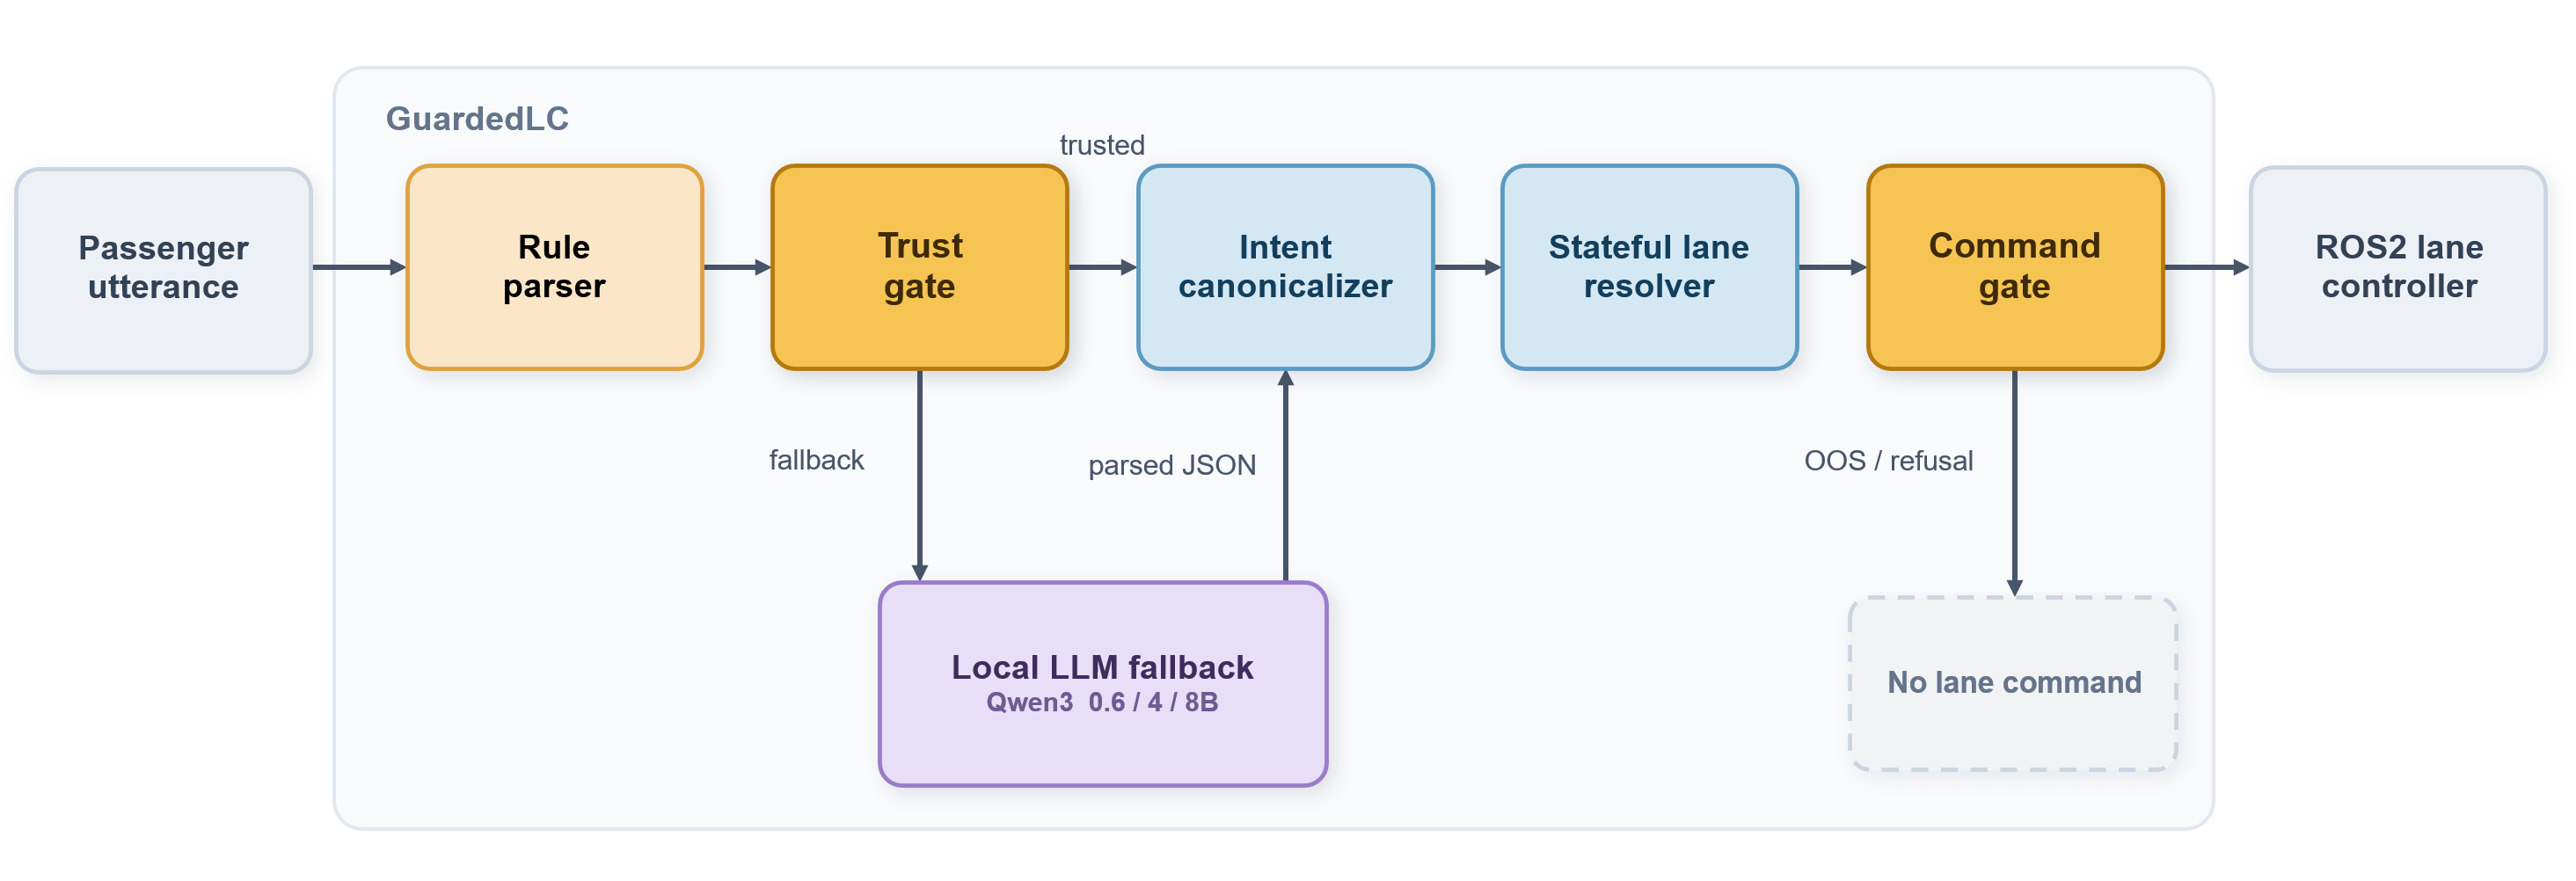
\includegraphics[width=0.88\textwidth]{fig1_pipeline.png}
\caption{\ours{} language-to-intent interface.}
\label{fig:pipeline}
\end{figure*}


\section{Introduction}
Language-conditioned driving is moving from passive scene understanding toward closed-loop planning, command interpretation, and policy execution. LMDrive integrates natural language with multimodal driving observations~\cite{lmdrive}; DriveLM, SimLingo, and BEVDriver extend this trend with graph reasoning, language-action alignment, or BEV grounding~\cite{drivelm,simlingo,bevdriver}. These works motivate a smaller but safety-critical deployment question: \emph{what should happen between a passenger utterance and the typed command interface consumed by a vehicle controller?}

This paper studies that boundary through a focused lane-change command interface. English utterances are parsed into symbolic lane intents and executed in a ROS2--Gazebo command pipeline~\cite{ros2,gazebo}. The interface is aligned with our lab's ROS2 autonomous-driving module lineage, including lane-change, lane-keeping path planning, path-tracking simulation, and modular AVP systems~\cite{skku_lanechange2024,skku_spline2025,skku_pathtracking2025,skku_avp2025}. The controlled two-lane setting isolates command-interface failures from perception, traffic, and route-planning confounders. A weak parser may miss paraphrases or spatial aliases, while an over-eager LLM may map ``do not change lanes'' to an active driving intent instead of the explicit hold-current type. ICR-Drive shows that paraphrase, ambiguity, noise, and misleading instructions can change closed-loop outcomes in language-conditioned agents~\cite{icrdrive}. Our contribution is complementary: \ours{} is not a driving policy; it emits typed lane-intent JSON for an existing controller while downstream perception, planning, and low-level control remain outside the claim.

We propose \emph{\ours}, a rule-first guarded router. The deterministic rule parser is trusted only for explicit target-lane changes, target-underspecified state-relative changes such as ``change lanes'', and keep-current/refusal commands. All other utterances are routed to a local Qwen3 model~\cite{qwen3}. The routing criterion is safety-typed rather than only confidence- or cost-driven: it asks whether an utterance type is allowed to produce a motion command, not only whether a model is likely to answer cheaply or accurately.

The evaluation separates parser correctness from vehicle behavior. Layer 1 (L1) measures parser-strict exact match and active-intent FP-OOS: a C6 refusal/OOS utterance is mapped to \texttt{CHANGE\_LANE} or \texttt{FOLLOW\_LANE} instead of a non-motion type. We separately report the stricter refusal-to-\texttt{CHANGE\_LANE} case. Layer 2 (L2) executes commands in a closed-loop simulator and measures final-lane correctness and command-level FP-OOS. Their difference, the \emph{rescue gap}, estimates how much the controller absorbs parser errors.

The contributions are: (i) a local Qwen3 capacity sweep showing a type-specific negative finding: larger LLM-only parsers improve average exact-match but increasingly map refusal/keep-current rows to active driving intents under P0 (1/10, 3/10, 6/10), while strict refusal-to-\texttt{CHANGE\_LANE} remains 0/10; (ii) a safety-typed routing criterion for language-to-intent command boundaries, with a held-out refusal stress test showing generalization within explicit-refusal rule coverage (8B: 7/15 active-intent FP-OOS reduced to 0/15) and coverage limits outside it; (iii) a two-layer evaluation framework that decomposes parser-strict correctness, active-intent FP-OOS, command-level FP-OOS, vehicle-loose success, and controller rescue through the rescue gap; and (iv) LC-Utt v1.0, a 150-utterance diagnostic benchmark with category-wise routing and C6 subtype traces.

\section{Related Work}
Language-conditioned driving and embodied VLA systems such as LMDrive, DriveLM, SimLingo, BEVDriver, and TrackVLA connect natural language with perception, reasoning, BEV grounding, trajectory planning, or visual tracking~\cite{lmdrive,drivelm,simlingo,bevdriver,trackvla}. Their primary evaluation unit is an end-to-end, perception-grounded, or trajectory-producing policy. \ours{} instead isolates the symbolic language-to-intent boundary that can precede either such a policy or a conventional controller.

Structured intermediate representations provide a related design pattern. SayCan grounds language choices in affordances, Code-as-Policies turns language into executable programs, and LaMPilot studies language-model programs for driving~\cite{saycan,codeaspolicies,lampilot}. \ours{} adopts structured output but narrows it to lane-intent JSON, allowing refusal and OOS decisions to be audited before motion publication; the model never emits continuous controls or trajectories.

Instruction robustness and external checks motivate the safety evaluation. ICR-Drive studies counterfactual instruction variants in end-to-end agents~\cite{icrdrive}, and RoboGuard checks LLM-generated robot plans against safety specifications~\cite{roboguard}. RouteLLM optimizes model selection for quality--cost trade-offs~\cite{routellm}, while Qwen3 makes local fallback models practical~\cite{qwen3}. Unlike quality--cost routing or plan-level verification, \ours{} asks whether an intent type may publish motion and separately reports parser output, command publication, and closed-loop behavior.

A deployed language interface also belongs to a broader systems stack. Mobile ad hoc network experiments show that real-time traffic performance can vary with node density~\cite{manet_density}; a review of Segment Anything discusses generality, resource limits, data bias, computational complexity, and real-world deployment issues in AI perception~\cite{segment_review}; and voice-cryptography work analyzes latency, energy, and platform trade-offs when protecting audio~\cite{voice_aes}. These concerns are complementary rather than evaluated here: our text-based study begins after an utterance is available and ends at symbolic lane-intent publication, leaving communication, perception, voice acquisition and security, and low-level control outside the claim.

\section{Methodology}
\subsection{Task, Intent Schema, and Benchmark}
The input is a user utterance $x$ and the output is structured JSON with intent, target lane, and auxiliary flags. The evaluated intent set is \{\texttt{CHANGE\_LANE}, \texttt{FOLLOW\_LANE}, \texttt{KEEP\_CURRENT\_LANE}, \texttt{QUERY\_STATE}, \texttt{UNKNOWN}\}; target lanes are \texttt{lane1}, \texttt{lane2}, or \texttt{null}. The implementation schema also includes \texttt{STOP} and \texttt{START} for the interactive GUI, but these intents are outside the LC-Utt evaluation. The parser never emits steering, throttle, or trajectories. In our fixed-direction track convention, inner/outer and left/right are deterministic lane identities rather than dynamically inferred ego-relative maneuvers: \texttt{lane1} maps to inner/left/first-lane expressions, and \texttt{lane2} maps to outer/right/second-lane expressions. Directionless state-relative requests keep \texttt{target\_lane=null} at L1; the L2 resolver selects the opposite lane from the current vehicle state.

LC-Utt v1.0 contains 150 utterances, balanced across six top-level categories (Table~\ref{tab:dataset}). C4 is intentionally named state-relative rather than arbitrary ambiguity: the maneuver intent is clear, but the target lane is underspecified. Therefore C4 L1 exact-match evaluates recognition of the state-relative intent and null target, not prediction of a concrete lane before state resolution. C6 combines two reported subtypes: 15 non-driving OOS utterances and 10 refusal/keep-current utterances. We keep them under one top-level C6 category because all should avoid publishing a motion-producing lane command, but we report subtype active-intent FP-OOS to separate ordinary OOS rejection from negation/refusal type errors. The utterances were authored as controlled diagnostic cases after the intent schema and categories were fixed; gold labels were assigned from the intended command template and manually checked against the schema. We did not use independent annotators, so LC-Utt should be read as a diagnostic benchmark rather than a naturalistic in-cabin corpus.

% Source: eval/lc_utt_v1.0.jsonl
\begin{table}[!t]
\centering
\caption{LC-Utt v1.0 Categories}
\label{tab:dataset}
\scriptsize
\setlength{\tabcolsep}{2.6pt}
\resizebox{\columnwidth}{!}{%
\begin{tabular}{@{}llrll@{}}
\toprule
ID & Category & $n$ & Purpose & Example \\
\midrule
C1 & Direct target & 25 & explicit lane-change target & ``change to lane 1'' \\
C2 & Polite/indirect & 25 & indirect requests and soft commands & ``could you move left?'' \\
C3 & Spatial aliases & 25 & left/right, inner/outer, first/second & ``take the inner lane'' \\
C4 & State-relative & 25 & target-underspecified lane-change intent & ``change lanes'' \\
C5 & Noisy/casual & 25 & typos, abbreviations, casual phrasing & ``chnge to lane1'' \\
C6 & OOS/refusal & 25 & 15 non-driving + 10 refusal/keep-current & ``do not change lanes'' \\
\bottomrule
\end{tabular}%
}
\end{table}


\subsection{Guarded Rule--LLM Router}
Fig.~\ref{fig:pipeline} summarizes the rule-first language-to-intent interface. A deterministic parser first proposes an intent, target lane, rule-specificity score $s_r(x)$, and rule class $f_r(x)$. The score is a heuristic string/alias specificity value, not a learned probability: exact lane-number matches receive high scores, unambiguous aliases receive lower scores, and conflicting or unmatched patterns are routed to the LLM. The implemented trust gate is
\begin{equation}
\operatorname{trust}(x)=
\begin{cases}
1, & s_r(x)\geq\tau \text{ and } f_r(x)\in\mathcal{C}_{\mathrm{trust}},\\
0, & \text{otherwise},
\end{cases}
\end{equation}
where $\tau=0.85$ and $\mathcal{C}_{\mathrm{trust}}$ contains only three rule classes: explicit-target lane changes, directionless state-relative lane changes, and keep-current/refusal commands. The two conditions play different roles: $s_r(x)$ checks that the string/alias match is specific enough, whereas $f_r(x)\in\mathcal{C}_{\mathrm{trust}}$ encodes whether that intent type is allowed to bypass the LLM and publish a lane command. Explicit targets are preserved: ``move over to lane 1'' is not collapsed to a null-target state-relative command. If $\operatorname{trust}(x)=0$, a local Qwen3 LLM parses the utterance with deterministic decoding.

The runtime path follows Fig.~\ref{fig:pipeline}: trusted rule outputs and LLM fallback JSON share the intent canonicalizer, the stateful resolver maps null-target changes from the current lane, and the command gate suppresses refusal/OOS outputs before the ROS2 lane controller. The offline evaluator, closed-loop runner, and GUI reuse the same trust and canonicalization functions.

The selected prompt is P0, the shortest baseline prompt in the ablation. It defines the JSON schema, lane aliases, and the rule that directionless changes should use a \texttt{null} target. In Section~\ref{sec:prompt}, we use prompt and threshold checks only as sensitivity analyses; the main evidence comes from the parser-level category breakdown and closed-loop evaluation.

\subsection{Evaluation Layers and Metrics}
L1 evaluates parser-strict exact match: both intent and target must match the gold label. L1 active-intent FP-OOS is measured on C6 and flags \texttt{CHANGE\_LANE} or \texttt{FOLLOW\_LANE} outputs for negative or out-of-scope commands; it is a typed parser error, not necessarily a published lane-change command. We also report strict refusal-to-\texttt{CHANGE\_LANE} on C6b. LLM-call rate is the fraction of utterances invoking the LLM.

L2 evaluates the same interface in Gazebo. Vehicle-loose correctness checks whether the final lane matches the expected behavior. Command FP-OOS is stricter than final-lane correctness: it flags whether a motion-producing lane command is published on C6. The rescue gap is
\begin{equation}
\Delta_{rescue}=Acc_{L2}-Acc_{L1},
\end{equation}
which measures downstream absorption of parser errors. Reset failures are simulator initialization failures before command execution; we report their count separately and do not treat them as language-interface failures. Because reset counts are not perfectly balanced across parsers, small L2 differences are interpreted conservatively and alongside command-level FP-OOS.

\section{Results}
\subsection{Experimental Setup}
L1 uses all 150 LC-Utt utterances with rule-only, LLM-only, and hybrid parsers across Qwen3-0.6B, 4B, and 8B; a final L1-only held-out stress test uses 30 unseen refusal utterances under P0. L2 nominal uses all 150 LC-Utt utterances for rule once, LLM-only 4B/8B, and hybrid 0.6B/4B/8B on a controlled two-lane Gazebo track. We omit 0.6B LLM-only in L2 because its L1 exact-match is far below both rule-only and hybrid; this omission limits claims about 0.6B LLM-only closed-loop behavior but does not affect the 4B/8B comparisons. Robustness uses a stratified subset of 50 utterances, hybrid only, warmup $\{1,3,5\}$s, and three replicates per capacity. The robustness sweep is a repeated-run timing-stability test of the deployed hybrid interface, not an independent expansion of the language corpus: its C6 portion contains 10 unique C6 utterances per capacity repeated under nine timing/replicate conditions. McNemar tests are exact and Holm-corrected over six L1 comparisons. Exact-match and vehicle-correctness CIs use category-stratified bootstrap, while gap/drop CIs use paired bootstrap over the same evaluation units. C6 active-intent FP-OOS CIs in L1 and nominal L2 command-FP CIs use exact binomial intervals over unique C6 utterances; repeated robustness runs are reported separately from unique-utterance evidence to avoid treating deterministic parser decisions as independent language samples. Reported latency includes rule routing and, when triggered, LLM invocation; absolute latency is system-local because hardware metadata were not logged, so the main latency claim is the relative reduction from invoking the LLM on 44\% of utterances in this balanced benchmark. All evaluated commands are text utterances; microphone capture, ASR errors, independently collected user commands, and real in-cabin interactions are not included. The reported counts are therefore diagnostic set outcomes rather than population-level failure rates.


\subsection{Layer 1: Accuracy, Safety, and Latency}
Table~\ref{tab:l1} reports L1 results. At 0.6B, the hybrid matches rule-only rather than improving on it, indicating that the weak fallback model contributes little beyond the trusted rule path. At 4B and 8B, however, the same architecture achieves the highest exact-match while reducing LLM calls from 100\% to 44\% on the balanced LC-Utt distribution. The main safety-relevant L1 pattern is a failure-type mismatch: LLM-only exact improves with capacity, but active-intent C6 FP-OOS worsens from 1/25 at 0.6B to 6/25 at 8B. These parser-level errors are active typed intents, mostly \texttt{FOLLOW\_LANE}, and should not be read as lane-change commands. In contrast, hybrid observes zero active-intent FP-OOS for every capacity in the evaluated C6 set; the 0/25 observation has an exact 95\% upper bound of 13.7\% per capacity.

Exact McNemar tests support the 0.6B and 4B hybrid exact-match gains over LLM-only (Holm $p=4.2\times10^{-17}$ and $1.5\times10^{-3}$). The very small 0.6B value mainly reflects the trusted rule path avoiding a weak LLM, not a hybrid-specific gain over rule-only. At 8B, the exact-match 6:0 row-level gain is nominal after Holm correction ($p=0.063$), so we state the 8B result as an observed directional improvement plus subtype-localized active-intent error interception, not as a statistically decisive exact-match gain.

% Sources: eval/results2/*/gpu/run1_results.csv, STATS_L1_BOOTSTRAP.csv, STATS_L1_FPOOS_BINOMIAL.csv
\begin{table}[!t]
\centering
\caption{Layer-1 Parser Results}
\label{tab:l1}
\scriptsize
\setlength{\tabcolsep}{2.2pt}
\resizebox{\columnwidth}{!}{%
\begin{tabular}{@{}llcccc@{}}
\toprule
Cap. & Parser & Exact [95\% CI] & C6 active FP [95\% CI] & LLM call & Lat. ms \\
\midrule
any & rule & 0.660 [0.593, 0.727] & 0/25 [0.000, 0.137] & 0\% & 0 \\
0.6B & LLM-only & 0.273 [0.213, 0.333] & 1/25 [0.001, 0.204] & 100\% & 492 \\
0.6B & GuardedLC & 0.660 [0.593, 0.727] & 0/25 [0.000, 0.137] & 44\% & 216 \\
4B & LLM-only & 0.860 [0.807, 0.913] & 3/25 [0.025, 0.312] & 100\% & 1482 \\
4B & GuardedLC & 0.940 [0.900, 0.973] & 0/25 [0.000, 0.137] & 44\% & 643 \\
8B & LLM-only & 0.927 [0.887, 0.967] & 6/25 [0.094, 0.451] & 100\% & 2336 \\
8B & GuardedLC & 0.967 [0.933, 0.993] & 0/25 [0.000, 0.137] & 44\% & 1005 \\
\bottomrule
\end{tabular}%
}
\end{table}


Fig.~\ref{fig:pareto} gives the latency--correctness view. The 4B and 8B hybrids have higher observed exact-match and lower mean latency than their LLM-only counterparts because only 44\% of LC-Utt utterances invoke the LLM. Since hardware metadata were not logged, latency is used only to support this relative call-reduction point on the benchmark distribution.

\begin{figure}[t]
\centering
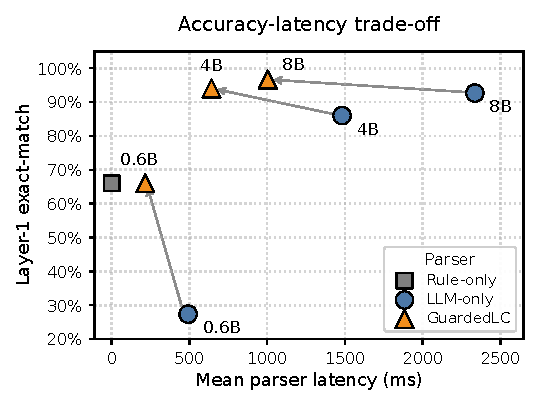
\includegraphics[width=0.96\columnwidth]{fig2_pareto.pdf}
\caption{Layer-1 accuracy--latency trade-off.}
\label{fig:pareto}
\end{figure}

Table~\ref{tab:c6_subtype} isolates the safety-relevant C6 cases. LLM-only active-intent FP-OOS is negation-specific rather than broad over-action: non-driving OOS has 0/15 FP-OOS for every capacity, while refusal/keep-current rises from 1/10 at 0.6B to 3/10 at 4B and 6/10 at 8B under P0. No evaluated refusal is mapped to \texttt{CHANGE\_LANE}; the observed L1 failure is that larger LLMs replace the explicit hold type with an active driving type, usually \texttt{FOLLOW\_LANE}. For example, 8B maps ``don't change lanes'' and ``no lane change'' to \texttt{FOLLOW\_LANE}, and maps ``stay in this lane'' to \texttt{FOLLOW\_LANE}/\texttt{lane1}. \ours{} observes 0/10 refusal/keep-current active-intent FP-OOS and 0/15 non-driving OOS FP-OOS for every capacity.

% Source: row-level C6 traces from eval/results2/*/gpu/run1_results.csv.
% C6a = u126--u140 non-driving OOS (n=15); C6b = u141--u150 refusal/keep-current (n=10).
% Active FP = CHANGE_LANE or FOLLOW_LANE on C6; strict change FP = CHANGE_LANE on C6b.
\begin{table}[!t]
\centering
\caption{C6 Subtype Layer-1 Errors Under P0}
\label{tab:c6_subtype}
\scriptsize
\setlength{\tabcolsep}{2.0pt}
\resizebox{\columnwidth}{!}{%
\begin{tabular}{@{}llcccc@{}}
\toprule
Cap. & Parser & C6a active & C6b active & C6b strict change & Total C6 active \\
\midrule
any & rule & 0/15 & 0/10 & 0/10 & 0/25 \\
0.6B & LLM-only & 0/15 & 1/10 & 0/10 & 1/25 \\
0.6B & GuardedLC & 0/15 & 0/10 & 0/10 & 0/25 \\
4B & LLM-only & 0/15 & 3/10 & 0/10 & 3/25 \\
4B & GuardedLC & 0/15 & 0/10 & 0/10 & 0/25 \\
8B & LLM-only & 0/15 & 6/10 & 0/10 & 6/25 \\
8B & GuardedLC & 0/15 & 0/10 & 0/10 & 0/25 \\
\bottomrule
\end{tabular}%
}
\end{table}


% Source: prompt ablation audit from eval/results2/prompt_ablation/*/run1_results.csv, summarized in data/prompt_c6b_active.csv.
\begin{table}[!t]
\centering
\caption{LLM-Only C6b Active-Intent FP-OOS Across Prompts}
\label{tab:prompt_c6b}
\scriptsize
\setlength{\tabcolsep}{5pt}
\begin{tabular}{@{}lccccc@{}}
\toprule
Cap. & P0 & P1 & P2 & P3 & Range \\
\midrule
0.6B & 1/10 & 3/10 & 0/10 & 1/10 & 0--3/10 \\
4B & 3/10 & 3/10 & 3/10 & 3/10 & 3/10 \\
8B & 6/10 & 5/10 & 4/10 & 3/10 & 3--6/10 \\
\bottomrule
\end{tabular}
\end{table}


\subsection{Category-wise L1 Behavior and Sensitivity}
\label{sec:prompt}
Table~\ref{tab:cat_l1} decomposes the aggregate L1 result and reports how often the hybrid gate routes each category to the LLM. The routing counts are capacity-independent because the deterministic trust gate runs before the LLM. Routing is utterance-level rather than category-level: for example, 10/25 C6 cases are explicit refusal/keep-current utterances that stay on the trusted rule path, while 15/25 non-driving OOS cases are routed to the LLM. Rule-only is strongest on state-relative and C6 non-motion cases, but it is weak on polite, spatial, and noisy language. The LLM path supplies most residual-language exact-match gain: at 4B, \ours{} raises C2/C3/C5 exact-match from the rule-only 0.56/0.48/0.36 to 0.96/0.88/0.96. At the same time, C6 exact-match and active-intent FP-OOS measure different risks. The 4B hybrid has one C6 exact-match miss, but it is a non-motion interpretation error; the active-intent FP-OOS count remains 0/25. Row-level C6 traces show that every LLM-only active-intent FP-OOS case at 0.6B/4B/8B falls inside the 10 utterances kept on the rule-trusted refusal/keep-current path, while none of the 15 LLM-routed non-driving OOS utterances produces FP-OOS. In LC-Utt v1.0 this subtype boundary coincides with the C6 routing partition, so subtype localization and routing interception are one observation viewed through semantic and routing labels rather than independent evidence.

% Sources: eval/results2/*/gpu/run1_results.csv; exact-match averaged over 25 utterances per category.
% The GLC LLM-route column is computed from the hybrid fallback field and is identical across capacities because the rule gate is deterministic.
\begin{table}[!t]
\centering
\caption{Category-Wise Layer-1 Exact Match and Routing}
\label{tab:cat_l1}
\scriptsize
\setlength{\tabcolsep}{1.6pt}
\resizebox{\columnwidth}{!}{%
\begin{tabular}{@{}lcccccc@{}}
\toprule
Category & GLC LLM-route & Rule & 4B LLM & 4B GLC & 8B LLM & 8B GLC \\
\midrule
C1 Direct target & 9/25 & 0.64 & 0.92 & 0.92 & 1.00 & 1.00 \\
C2 Polite/indirect & 11/25 & 0.56 & 0.80 & 0.96 & 0.96 & 0.96 \\
C3 Spatial aliases & 13/25 & 0.48 & 0.72 & 0.88 & 0.88 & 0.88 \\
C4 State-relative & 2/25 & 0.92 & 0.96 & 0.96 & 1.00 & 1.00 \\
C5 Noisy/casual & 16/25 & 0.36 & 0.92 & 0.96 & 0.96 & 0.96 \\
C6 OOS/refusal & 15/25 & 1.00 & 0.84 & 0.96 & 0.76 & 1.00 \\
\bottomrule
\end{tabular}%
}
\end{table}


Prompt and threshold checks were used as sensitivity analyses rather than primary evidence. Table~\ref{tab:prompt_c6b} shows that the P0 1/10--3/10--6/10 pattern is the clearest instance; across P0--P3 the effect size is prompt-dependent, with 4B stable at 3/10 and 8B ranging from 3/10 to 6/10, while non-driving OOS remains 0/15 in all twelve prompt-capacity conditions. P0 and P2 tie in average hybrid exact-match, but P2/P3 introduce a null-target bias in the 0.6B LLM-only parser, so P0 is used for L2. A trust-threshold sweep shows a stable plateau for $\tau\le0.87$; when the threshold disables rule-trusted outputs, active-intent FP-OOS returns toward LLM-only behavior. Thus the evaluated FP-OOS interception is caused by the trusted intent set, especially explicit refusal/keep-current handling, rather than by threshold tuning alone.

As a final L1 stress test, we authored 30 unseen refusals with gold \texttt{KEEP\_CURRENT\_LANE} and no text overlap with LC-Utt v1.0. We curated this stress set to balance 15 explicit refusals reachable by the rule's negative/keep-current patterns (H1) and 15 paraphrased refusals that escape those patterns and route to the LLM (H2), with subset membership validated using the actual rule parser. On H1, \ours{} keeps all 15 utterances on the trusted path and emits 0/15 active-intent FP-OOS at every capacity, whereas 8B LLM-only emits 7/15 active-intent FP-OOS, including one strict refusal-to-\texttt{CHANGE\_LANE} error (``do not change to the other lane'') and two targeted-active errors (``i want to stay in this lane'' and ``just keep this lane'' $\rightarrow$ \texttt{FOLLOW\_LANE}/\texttt{lane1}). On H2, all utterances route to the LLM, so \ours{} matches LLM-only: active-intent FP-OOS is 1/15, 1/15, and 3/15 for 0.6B, 4B, and 8B, respectively, with 0/15 targeted-active errors. The stress test shows both generalization within explicit-refusal rule coverage and the coverage limit on paraphrased refusal.

\subsection{Layer 2: Closed-Loop Behavior and Rescue Gap}
Table~\ref{tab:l2} reports nominal L2 results. The L2 numbers are used mainly to expose downstream absorption: most parsers reach high vehicle-loose correctness, including rule-only, but their parser traces and command-level FP-OOS differ. The 8B LLM-only baseline publishes one motion command on C6 despite strong L1 exact-match, while no hybrid does so in the nominal run. This is the actual command-publication safety event in the evaluation. The distinction between L1 active-intent FP-OOS and command FP-OOS matters because most parser-level active-intent errors, especially \texttt{FOLLOW\_LANE} with \texttt{target\_lane=null}, do not become motion commands after stateful resolution.

% Sources: L2_NOMINAL_TABLE.csv, STATS_L2_NOMINAL_BOOTSTRAP.csv, STATS_L2_FPOOS_BINOMIAL.csv
\begin{table}[!t]
\centering
\caption{Nominal Layer-2 Closed-Loop Results}
\label{tab:l2}
\scriptsize
\setlength{\tabcolsep}{1.55pt}
\resizebox{\columnwidth}{!}{%
\begin{tabular}{@{}llcccccc@{}}
\toprule
Cap. & Parser & L1 & L2 [95\% CI] & Gap [95\% CI] & Call & Cmd FP [95\% CI] & Valid/Reset \\
\midrule
any & rule & 0.660 & 0.973 [0.947, 0.993] & +0.313 [0.247, 0.380] & 0\% & 0/25 [0.000, 0.137] & 149/1 \\
0.6B & GuardedLC & 0.660 & 0.900 [0.853, 0.940] & +0.240 [0.180, 0.307] & 44\% & 0/25 [0.000, 0.137] & 146/4 \\
4B & LLM-only & 0.860 & 0.987 [0.967, 1.000] & +0.127 [0.080, 0.180] & 100\% & 0/25 [0.000, 0.137] & 145/5 \\
4B & GuardedLC & 0.940 & 0.993 [0.980, 1.000] & +0.053 [0.020, 0.093] & 44\% & 0/25 [0.000, 0.137] & 141/9 \\
8B & LLM-only & 0.927 & 0.993 [0.980, 1.000] & +0.067 [0.033, 0.107] & 100\% & 1/25 [0.001, 0.204] & 136/14 \\
8B & GuardedLC & 0.967 & 1.000 & +0.033 [0.007, 0.067] & 44\% & 0/25 [0.000, 0.137] & 138/12 \\
\bottomrule
\end{tabular}%
}
\end{table}


The rescue gap provides the main interpretive tool. Rule-only has high L2 correctness (0.973) despite low L1 exact (0.660), yielding a +31.3 pp gap; the 4B and 8B hybrids reduce the gap to +5.3 pp and +3.3 pp. This shows why final-lane correctness alone can conflate a correct language interface with a forgiving downstream controller.
\subsection{Robustness Across Command Timing}
The robustness sweep checks whether nominal L2 behavior is a timing artifact for the deployed hybrid interface. Table~\ref{tab:robust} summarizes 1,350 repeated executions over subset50, three warmups, and three replicates per capacity. Observed worst-drop is 2 pp for 0.6B and 0 pp for 4B/8B; paired bootstrap gives upper bounds of 6 pp for 0.6B/4B and 0 for 8B. Because the same 10 C6 utterances per capacity are repeated under timing conditions, the no-FP result is command-timing stability evidence rather than a larger independent language sample.


% Sources: L2_ROBUSTNESS_BY_CAPACITY.csv, STATS_L2_ROBUSTNESS_BOOTSTRAP.csv, STATS_L2_ROBUSTNESS_SUMMARY.csv
\begin{table}[!t]
\centering
\caption{Layer-2 Robustness on Subset50}
\label{tab:robust}
\scriptsize
\setlength{\tabcolsep}{1.5pt}
\resizebox{\columnwidth}{!}{%
\begin{tabular}{@{}lcccccc@{}}
\toprule
Cap. & Ref. & Mean L2 [95\% CI] & Min--Max & Drop [95\% CI] & C6 Cmd FP & Reset \\
\midrule
0.6B & 0.900 & 0.898 [0.800, 0.976] & 0.880--0.900 & 0.020 [0.000, 0.060] & 0/10 uniq.; 0/90 runs & 14.4\% \\
4B & 0.980 & 0.996 [0.989, 1.000] & 0.980--1.000 & 0.000 [0.000, 0.060] & 0/10 uniq.; 0/90 runs & 3.6\% \\
8B & 1.000 & 1.000 & 1.000--1.000 & 0.000 & 0/10 uniq.; 0/90 runs & 5.8\% \\
\bottomrule
\end{tabular}%
}
\end{table}


The 8B hybrid is exact on all 450 parser-level robustness executions and correct on all 450 vehicle-level executions, whereas 0.6B hybrid has parser-exact 333/450 but L2 correct 404/450. This again shows that vehicle-loose correctness can make weak parsers look stronger than they are. Reset failures occur before any lane command is published and are logged separately; their unequal rates are another reason to read L2 together with parser-level metrics.



\subsection{Discussion of Scope and Differentiation}
The main transferable result is type-specific: larger local LLMs improve average parsing yet can worsen refusal/keep-current active-intent errors. This supports reporting failure type and command publication rather than exact-match alone. The one nominal L2 command FP and the author-generated held-out set remain diagnostic, but the latter shows both the benefit and limit of rule coverage: explicit H1 refusals are intercepted, while H2 paraphrases inherit LLM errors. The result does not imply that rules can replace LLMs; rule-only exact-match is 0.660, and the LLM remains necessary for polite, spatial, noisy, and residual OOS language. Rescue gap further shows why high final-lane success can reflect downstream controller absorption rather than a correct language interface.

\subsection{Threats to Validity}
LC-Utt covers only lane-change commands on a controlled two-lane track; it does not establish robustness to dialogue, navigation, traffic negotiation, or perception-heavy maneuvers. Both language sets were authored by us, without independent annotators, user-collected commands, ASR corruption, or in-cabin interaction, and the rule classes are not independent of the benchmark categories. Zero FP-OOS therefore does not establish broad paraphrase coverage or population prevalence. The timing sweep repeats the same language items, the controller is deterministic and forgiving, and reset rates are unequal. Finally, results are limited to Qwen3 and system-local latency; future deployment studies should report hardware, runtime, quantization, warm-up policy, and p95/p99 latency.

\balance
\section{Conclusion}
\ours{} exposes command-boundary failures hidden by aggregate parser or vehicle metrics. Under P0, LLM-only exact-match rises with capacity while refusal/keep-current active-intent errors rise from 1/10 to 3/10 to 6/10. The 4B/8B hybrids improve observed exact-match, reduce LLM calls to 44\%, and record zero diagnostic C6 parser- and command-level FP-OOS by retaining explicit refusals on the trusted path. The held-out test bounds this result: rule-covered H1 refusals are intercepted, while H2 paraphrases inherit LLM errors. These author-generated text results are diagnostic, not a naturalistic safety guarantee. Future work should evaluate independently collected and ASR-corrupted commands, real in-cabin interactions, multiple maneuvers, scene-aware checks, and hardware-logged tail latency.

\section*{Acknowledgment}
This work was supported by Korea Institute for Advancement of Technology (KIAT) grant funded by the Korea Government (MOTIE) (RS-2024-00415938, HRD Program for Industrial Innovation).

\begin{thebibliography}{99}
\setlength{\itemsep}{0pt}
\setlength{\parsep}{0pt}

\bibitem{lmdrive}
H. Shao \textit{et al.}, ``LMDrive: Closed-loop end-to-end driving with large language models,'' in \textit{Proc. IEEE/CVF CVPR}, 2024, pp. 15120--15130, doi: 10.1109/CVPR52733.2024.01432.

\bibitem{drivelm}
C. Sima \textit{et al.}, ``DriveLM: Driving with graph visual question answering,'' in \textit{Proc. ECCV}, 2024.

\bibitem{simlingo}
K. Renz, L. Chen, E. Arani, and O. Sinavski, ``SimLingo: Vision-only closed-loop autonomous driving with language-action alignment,'' in \textit{Proc. IEEE/CVF CVPR}, 2025, pp. 11993--12003.

\bibitem{bevdriver}
K. Winter, M. Azer, and F. B. Flohr, ``BEVDriver: Leveraging BEV maps in LLMs for robust closed-loop driving,'' in \textit{Proc. IEEE/RSJ IROS}, 2025, doi: 10.1109/IROS60139.2025.11247237.

\bibitem{ros2}
S. Macenski, T. Foote, B. Gerkey, C. Lalancette, and W. Woodall, ``Robot Operating System 2: Design, architecture, and uses in the wild,'' \textit{Science Robotics}, vol. 7, no. 66, eabm6074, 2022.

\bibitem{gazebo}
N. Koenig and A. Howard, ``Design and use paradigms for Gazebo, an open-source multi-robot simulator,'' in \textit{Proc. IEEE/RSJ IROS}, 2004, pp. 2149--2154.

\bibitem{skku_lanechange2024}
Y. G. Choi, H. Hong, and J. W. Jeon, ``Implementation of a lane change system module using YOLOv8 based on ROS2: Porting to Jetson Orin Nano and performance analysis,'' in \textit{Proc. APAC22 Asia Pacific Automotive Engineering Conf.}, 2024.

\bibitem{skku_spline2025}
H. K. Hong, J. S. Lee, E. H. Kim, Y. K. Choi, Y. H. Seo, and J. W. Jeon, ``A spline-based path planning for lane keeping in autonomous vehicles,'' in \textit{Proc. ICMRE}, 2025, pp. 55--59, doi: 10.1109/ICMRE64970.2025.10976287.

\bibitem{skku_pathtracking2025}
S. H. Jung \textit{et al.}, ``Beyond proportional control: A comparative ROS2 simulation on path tracking with PID+Pure Pursuit,'' in \textit{Proc. IEEE/IEIE ICCE--Asia}, 2025, doi: 10.1109/ICCE-Asia67487.2025.11263600.

\bibitem{skku_avp2025}
Y. G. Choi \textit{et al.}, ``Infrastructure sensor-based modular autonomous valet parking system using ROS 2,'' in \textit{Proc. ITC--CSCC}, 2025, doi: 10.1109/ITC-CSCC66376.2025.11137602.

\bibitem{icrdrive}
K. Hamid, C. Cui, and N. Liang, ``ICR-Drive: Instruction counterfactual robustness for end-to-end language-driven autonomous driving,'' in \textit{Proc. IEEE/CVF CVPR Workshops}, 2026, pp. 872--880.

\bibitem{qwen3}
A. Yang \textit{et al.}, ``Qwen3 technical report,'' \textit{arXiv:2505.09388}, 2025.

\bibitem{trackvla}
S. Wang \textit{et al.}, ``TrackVLA: Embodied visual tracking in the wild,'' in \textit{Proc. 9th Conf. Robot Learning}, PMLR, vol. 305, 2025, pp. 4139--4164.

\bibitem{saycan}
M. Ahn \textit{et al.}, ``Do As I Can, Not As I Say: Grounding language in robotic affordances,'' in \textit{Proc. 6th Conf. Robot Learning}, PMLR, vol. 205, 2023, pp. 287--318.

\bibitem{codeaspolicies}
J. Liang \textit{et al.}, ``Code as policies: Language model programs for embodied control,'' in \textit{Proc. IEEE ICRA}, 2023, pp. 9493--9500.

\bibitem{lampilot}
Y. Ma \textit{et al.}, ``LaMPilot: An open benchmark dataset for autonomous driving with language model programs,'' in \textit{Proc. IEEE/CVF CVPR}, 2024.

\bibitem{roboguard}
Z. Ravichandran, A. Robey, V. Kumar, G. J. Pappas, and H. Hassani, ``Safety guardrails for LLM-enabled robots,'' \textit{IEEE Robotics and Automation Letters}, vol. 11, no. 4, pp. 4649--4656, 2026.

\bibitem{routellm}
I. Ong \textit{et al.}, ``RouteLLM: Learning to route LLMs with preference data,'' in \textit{Proc. ICLR}, 2025.

\bibitem{manet_density}
F. Hazzaa, S. Yousef, N. H. Ali, and E. Sanchez, ``The effect of nodes density on real time traffic in mobile ad hoc network,'' in \textit{Proc. 2019 IEEE 12th Int. Conf. Global Security, Safety and Sustainability (ICGS3)}, London, UK, 2019, pp. 209--212, doi: 10.1109/ICGS3.2019.8688314.

\bibitem{segment_review}
F. Hazzaa, I. Udoidiong, A. Qashou, and S. Yousef, ``Segment Anything: A review,'' \textit{Mesopotamian Journal of Computer Science}, vol. 2024, pp. 150--161, 2024, doi: 10.58496/MJCSC/2024/012.

\bibitem{voice_aes}
F. Hazzaa, A. Qashou, I. I. Al Barazanchi, R. Sekhar, P. Shah, M. Bachute, and A. S. Abdulbaqi, ``Performance analysis of advanced encryption standards for voice cryptography with multiple patterns,'' \textit{International Journal of Safety and Security Engineering}, vol. 14, no. 5, pp. 1439--1446, 2024, doi: 10.18280/ijsse.140511.

\end{thebibliography}

\end{document}
